\documentclass[a4paper,UTF8]{article}
\usepackage{ctex}
\usepackage[margin=1.25in]{geometry}
\usepackage{color}
\usepackage{graphicx}
\usepackage{amssymb}
\usepackage{amsmath}
\usepackage{amsthm}
%\usepackage[thmmarks, amsmath, thref]{ntheorem}
\theoremstyle{definition}
\newtheorem*{solution}{Solution}
\newtheorem*{prove}{Proof}
\usepackage{multirow}
\usepackage{url}
\usepackage[colorlinks,urlcolor=blue]{hyperref}
\usepackage{enumerate}
\setcounter{secnumdepth}{4}
\usepackage{float}
\usepackage{listings}
\usepackage{xcolor}
\lstset{
	%backgroundcolor=\color{red!50!green!50!blue!50},%代码块背景色为浅灰色
	rulesepcolor= \color{gray}, %代码块边框颜色
	breaklines=true,  %代码过长则换行
	numbers=left, %行号在左侧显示
	numberstyle= \small,%行号字体
	%keywordstyle= \color{red},%关键字颜色
	commentstyle=\color{gray}, %注释颜色
	frame=shadowbox%用方框框住代码块
}
\renewcommand\refname{参考文献}
%--

%--
\begin{document}
\title{\textbf{《计算机图形学》 5月报告 }}
\author{学号,姓名,\href{mailto:xxx@xxx.com}{171240511@smail.nju.edu.cn}}
\maketitle

\section{综述}
在老师所给框架代码上进行修改完善,完成了所有要求的指令输入输出,GUI界面实现了所CLI部分的所有功能,包括设置画笔颜色、重置画布、保存画布、两种算法绘制线段、两种算法绘制多边形、绘制椭圆、两种算法绘制曲线、平移、旋转、缩放和两种算法裁剪线段.\\
\indent 额外实现了点击画布右、下、右下角边框调整画布大小.
\section{算法介绍}
\subsection{绘制线段}
\subsubsection{DDA算法} 
基本思想是记下起点,然后让长的一边变量不断加一,短的一边则不断加斜率乘1后近似为int值.代码参照\cite{rog_2002}.
\subsubsection{Bresenham算法} 
基本思想其实和DDA是一样的.只是Bresenham算法通过变形避免了浮点运算.这样一来,既提高了运算的效率,又避免了浮点数不断累加造成的长线段误差.所以本质上,Bresenham是DDA算法的优化形式.代码参照\cite{rog_2002}.
\subsubsection{代码处理}
\begin{itemize}
\item 特判使得能够处理两端点相等的情况.
\item 因为讲义中说不要求像素级一致,所以和伪代码一样只亮一边端点,即线段点的范围$[P_0,P_1)$.
\end{itemize}

\subsection{绘制多边形}
默认指令中的点是排好序的, 直接调用线段绘制算法按顺序连点.

\subsection{绘制椭圆}
\indent 使用ppt上的中点椭圆算法, 先画出1/4椭圆, 然后对称. 画1/4椭圆时,根据是否到达切线斜率为-1的位置, 来判断选点的方向是基于x还是基于y, 再根据实际椭圆上的点离哪个点更近取近似.\\
\indent 实际代码要先求出中心和长短轴, 然后以中心为原点求点, 再映射回原来的坐标系.\\
\indent 对称的时候考虑了x轴和y轴上的特例, 不然x=0和y=0的点对称后相当于1个点出现了两次.\\
\indent 代码流程参考书上ppt相关部分.

\subsection{绘制曲线}
\subsubsection{Bezier曲线} 
书上给出了Bezier曲线关于控制点的参数方程和矩阵形式, 但直接这样计算参数u对应的点效率太低, 于是又给出了de Casteljau递推算法来快速计算一个u值对应的曲线上点的坐标.\\
\indent 有了这个递推算法后, 由于参数u位于[0,1]之间,理论上我们只要将[0,1]分割的足够小,就可以得到精度足够高的一条Bezier曲线.\\
\indent 但这样分割, 为了确保精度, 我们往往要将步长设置的非常小, 从而导致计算次数过多. 于是书上给出了一种二分逼近的办法.也就是每次先计算u=1/2处的点, 然后用这个点将曲线分为两段, 再对这两段曲线进行u值的二分, 重复这个二分的操作, 最后每段曲线的控制多边形会很接近理论曲线, 就可以直接拿控制多边形当作实际曲线.\\
\indent 实现参考\cite{sun_2006}中6.3.3和6.3.4.
\subsubsection{B-spline曲线}
B样条曲线的绘制本质上和Bezier没什么不同, 都是要根据递推式求参数u对应的离散点. 但具体实现起来还是有所不同的.\\
\indent B样条曲线实际上是按照次数进行分段绘制的, k次B样条就是每k+1个控制点一段, 相邻两段有k个公共控制点, 这也解释了为什么它具有局部性.\\
\indent 不过, 由于它的控制多边形不像Bezier曲线那样可以随着二分不断逼近, 在具体绘制一段B样条曲线时, 只能设置步长密集取点, 这既导致了步长取密时曲线会变粗(重叠部分), 也导致了效率的降低.\\
\indent 实现参考\cite{bspline_web}.
\subsubsection{代码处理}
B-spline曲线绘制其中一段时, 目前选择取100个离散点, 再往大取GUI绘制时就会很卡.

\subsection{平移}
\indent 平移部分参考ppt, 直接令各图形的控制点偏移[dx,dy]即可.

\subsection{旋转}
\indent 旋转部分参考ppt, 直接套用公式, 各图形的控制点相对于旋转中心[x,y]顺时针旋转r度即可.

\subsection{缩放}
\indent 缩放部分参考ppt, 直接套用公式, 控制点相对于缩放中心[x,y]缩放s倍即可.

\subsection{裁剪}
\subsubsection{Cohen-Sutherland算} 
这个算法的特别之处在于位运算的思想,用4位二进制数表示左右上下四个位置的是否. 接着再分类讨论不同情况下线段裁剪时, 就可以用位运算来判断怎么裁剪线段. 它会重复裁剪直到线段完全在窗口内或者完全在窗口外.
代码参考\cite{cohen_web}.\\
\subsubsection{Liang-Barskey算法法} 
这个算法不同于Cohen-Sutherland算法, 它希望一步直接将线段裁剪出来, 而不是重复裁剪.
它用$P=P_1+u*(P2-P1)$来表示直线P, 并分情况判断和裁剪窗口相交点处的$u_1,u_2$值, 根据$u_1,u_2$的情况来判断结果.
代码参考\cite{liang_web}和ppt.

\section{系统介绍}
\subsection{CLI框架}
沿用了老师的框架, 每次进行绘制图元或编辑图元操作时, 将需要的绘制信息储存在字典item\_dict中, 等到save\_Canvas时再根据每个item的item\_type, 调用相应算法计算图元的像素点, 并修改canvas中的值.
\subsection{GUI框架}
gui部分沿用了老师MainWindow(继承QMainWindow)作为主窗口, MyCanvas(继承QGraphicsView)作为画布, MyItem(继承QGraphicsItem)储存图元信息的框架.\\
\indent 原始代码由于点击绘制图元和在画布上press mouse时都调用get\_id方法, 使item\_cnt加1,因此图元编号并不连续. 对此进行了修改, 令get\_id方法不修改item\_cnt, 另外声明方法id\_inc来修改item\_cnt.\\
\indent 窗口布局情况如下图:
\begin{itemize}
	\item 最上面是菜单栏,由self.menuBar()方法返回, 可以进行设置画笔颜色等操作.
	\item 下面一行是编辑工具栏,由self.addToolBar方法添加, 可以对图元进行平移等操作.
	\item 左边是绘图工具栏,由self.addToolBar方法添加, 可以选择要绘制的图元类型及算法.
	\item 右边窗口显示图元类型及编号, 由self.list\_widget()返回, 点击可以用于选择图元.
	\item 下方状态栏, 由self.statusBar()方法返回, 显示当前在进行什么操作.
	\item 最中间的则是画布区域, 定义MyCanvas类, 可以用鼠标操作绘图.
\end{itemize}
\begin{figure}[H]
	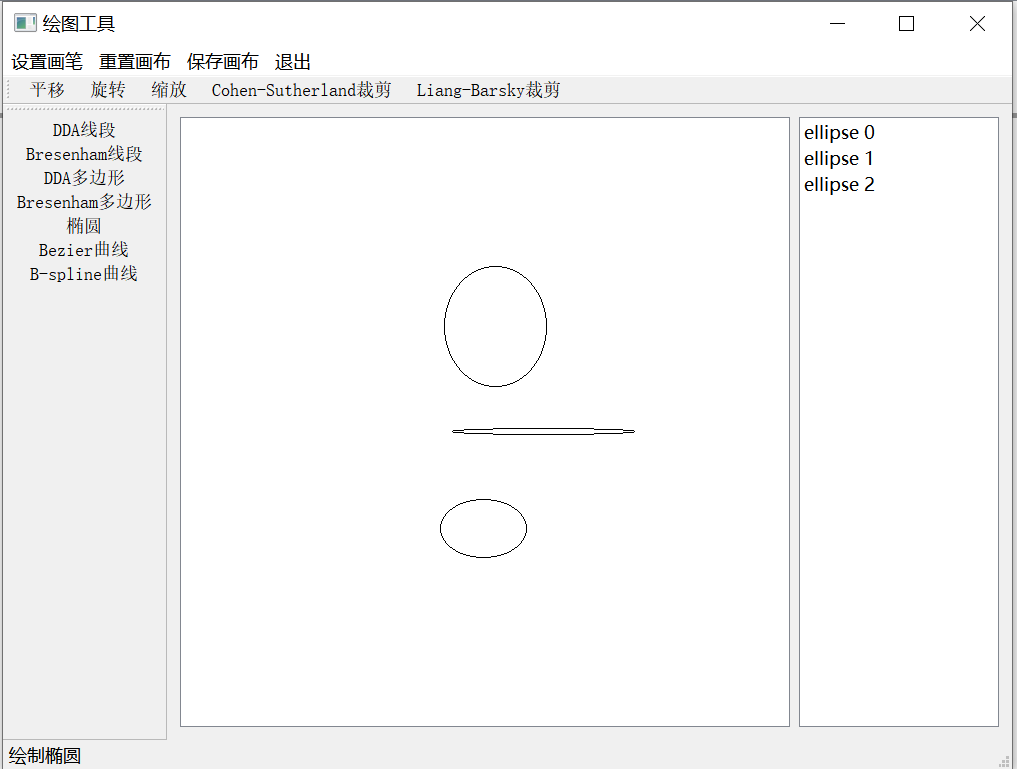
\includegraphics[width=5in,height=3in]{total.png}
\end{figure}
\subsection{GUI功能}
\subsubsection{菜单栏}
画笔颜色选择参考了\cite{pyqt5_ch}, 利用QColorDialog唤出调色板, 将选取的颜色值存在全局变量g\_penColor中, 每次要绘制图元的时候将g\_penColor作为画笔颜色, 关键代码如下:\\
\begin{lstlisting}[language={python}]
global g_penColor
color = QColorDialog.getColor()
g_penColor = color
\end{lstlisting}
\indent\\
\indent 重置画布操作也参考了\cite{pyqt5_ch}, 调用两次QInputDialog获取新画布的x,y轴大小, 然后清空画布和场景, 初始化各个变量.\\
\indent 保存画布的代码参考了\cite{save_canvas}, 利用QFileDialog.getSaveFileName输入要生成文件的目录和名字, 然后再用QGraphicsScene的render方法将画布的内容储存到QPixmap类中, 最后用QPixmap类的save方法生成文件.关键代码如下:\\
\begin{lstlisting}[language={python}]
fname = QFileDialog.getSaveFileName(self, 'Save file',\
'/home/output/default','Image files (*.bmp)')        
#cancel save
if(fname[0]==''):
    return
# Get QRectF
rect = self.scene.sceneRect()
# Create a pixmap, fill with white color
pixmap = QPixmap(g_width, g_height)
# set background white
pixmap.fill(QColor(255,255,255))
# painter
painter = QPainter(pixmap)
# Render scene to the pixmap
self.scene.render(painter, rect, rect)
painter.end()
# save bmp file
pixmap.save(fname[0])    
\end{lstlisting}
\subsubsection{绘图工具栏}
绘制线段和绘制椭圆其实是类似的, 都是先在mousePressEvent中记录一个端点, 然后在mouseMoveEvent中记录另一个端点, 然后利用updateScene方法更新画布, 这样在MyItem类中会自动调用paint方法绘制图形.\\
\indent 绘制多边形又和绘制曲线类似, 都是要输入多个点集, 就添加一个全局变量g\_draw\_finish来判断绘制是否输入结束.具体来说, 多边形绘制时如果最后一个点在起始点5$\times$5范围内, 就闭合, g\_draw\_finish=1. 否则, 就和曲线绘制一样, 一直等到下一个任意操作(比如平移)时再调用check\_finish方法检测并处理未完成图元.\\
\indent 注意, 绘制曲线时, 每次新控制点加入到末端控制点后面而非前面, 关键代码如下:\\
\begin{lstlisting}[language={python}]
le = len(self.temp_item.p_list)
if le <= 2: 
    self.temp_item.p_list[-1] = [x, y]
else:
    self.temp_item.p_list[-2] = [x, y]
\end{lstlisting}
\subsubsection{编辑工具栏}
\indent 任何编辑操作前都要点击右边窗口选择图元.\\
\indent 为了处理不同的编辑操作, 在MyItem中添加str类型的trans\_type成员, 用于判断编辑操作.\\
\indent 平移操作时, 鼠标按下的点为[x0,y0], 移动时为[x1,y1], 计算出dx,dy并paint.\\
\indent 旋转操作需要鼠标点击两次, 第一次点击确定了旋转中心坐标, 记录在MyItem的center中, 第二次点击和移动则确定了两个新的点存在MyItem的poi和poi1中,这时poi1-center和poi-center的夹角即为旋转角.注意椭圆不能旋转, 关键代码如下:\\
\begin{lstlisting}[language={python}]
if self.item_type == 'ellipse':
    print("Can't rotate ellipse")
    return 
if self.param_cnt == 2:
    # center and poi, poi1 all gotten
    theta = angle([self.center, self.poi], [self.center, self.poi1])
    new_p_list = alg.rotate(self.p_list, \
              self.center[0], self.center[1], theta)
\end{lstlisting}
\indent\\
\indent 编辑时有些操作参数较多,需要点击两次,比如旋转,这时如果点击一次就切走做别的,第一次点击选择的点仍然会保留在对应item中.但是每次进行编辑操作前都会调用selectedTransClear()方法,确保选择的item的相应参数恢复到初始状态.\\
\indent 缩放基本的实现思路和旋转一致, 先确定缩放中心, 再根据两线段x方向比值确定缩放倍数.\\
\indent 裁剪操作时,绘制裁剪窗口,并高亮窗口内线段,关键代码如下: \\
\begin{lstlisting}[language={python}]
# draw the clip window
painter.setPen(QColor(255, 0, 0))
painter.drawRect( self.regionRect([self.center,self.poi]) )                 
tmp_p_list = alg.clip(self.p_list, self.center[0], self.center[1], self.poi[0], self.poi[1], self.trans_algorithm)
if tmp_p_list != []:
    # highlight the line in clip window
    tmp_pixels = draw(tmp_p_list,self.algorithm)
    painter.setPen(QColor(255, 0, 0))
    for p in tmp_pixels:
        thick_draw_point(painter, p)
\end{lstlisting}
\indent 如果裁剪对象不是线段, 则不起作用. 而如果裁剪后线段什么点也没剩下,仍然保留QListWiget中该图元,但是无法对其进行任何操作.
\subsection{额外功能}
目前实现的额外功能是点击画布右、下、右下角边框后拖动调整画布大小, 这个功能并不会对正在进行的绘制有影响. 具体是通过MyCanvas中的is\_image\_scaling来判断情况的, 关键代码如下:\\
\begin{lstlisting}[language={python}]
if g_width-5 <= x <= g_width+5 and g_height-5 <= y <= g_height+5:
    self.is_image_scaling = 3  
elif g_width-5 <= x <= g_width+5:  
    self.is_image_scaling = 1  
elif g_height-5 <= y <= g_height+5:  
    self.is_image_scaling = 2
\end{lstlisting}
\section{总结}
\subsection{遇到的一些问题}
\begin{itemize}
	\item gui中sys.exit(app.exec\_())改为app.exec\_(),自己手动退出,不然Spyder运行手动退出时会报错.
	此外,还得加上del app,不然重新运行的时候也会有点问题.参考\cite{exit}
	
	\item 框架代码是鼠标一动就将MyItem中的图元绘制,
	这导致绘制直线的时候直线随着拖动不断绘制,这包括了最开始端点重合的情况,
	对于DDA会出现除0错误,因此要特判.
	
	\item 画笔颜色选择分两步,一个是会用QColorDialog调出调色版,另一个是要将画笔颜色传给MyItem,我用全局变量g\_penColor传递.
\end{itemize}
1.多边形没画完就edit不会自动终止\\
2.添加了不能裁剪非线段的提示\\
3.添加了点击画布选择图元, 试图使用QGraphicsScene的itemAt方法,发现两个item重叠多的时候很难选,于是改成记录图元的所有点,与鼠标点击的坐标逐一比对
\bibliographystyle{plain}%
%"xxx" should be your citing file's name.
\bibliography{cgref}
\end{document}